% Options for packages loaded elsewhere
\PassOptionsToPackage{unicode}{hyperref}
\PassOptionsToPackage{hyphens}{url}
%
\documentclass[
  oneside]{book}
\usepackage{amsmath,amssymb}
\usepackage{lmodern}
\usepackage{iftex}
\ifPDFTeX
  \usepackage[T1]{fontenc}
  \usepackage[utf8]{inputenc}
  \usepackage{textcomp} % provide euro and other symbols
\else % if luatex or xetex
  \usepackage{unicode-math}
  \defaultfontfeatures{Scale=MatchLowercase}
  \defaultfontfeatures[\rmfamily]{Ligatures=TeX,Scale=1}
\fi
% Use upquote if available, for straight quotes in verbatim environments
\IfFileExists{upquote.sty}{\usepackage{upquote}}{}
\IfFileExists{microtype.sty}{% use microtype if available
  \usepackage[]{microtype}
  \UseMicrotypeSet[protrusion]{basicmath} % disable protrusion for tt fonts
}{}
\makeatletter
\@ifundefined{KOMAClassName}{% if non-KOMA class
  \IfFileExists{parskip.sty}{%
    \usepackage{parskip}
  }{% else
    \setlength{\parindent}{0pt}
    \setlength{\parskip}{6pt plus 2pt minus 1pt}}
}{% if KOMA class
  \KOMAoptions{parskip=half}}
\makeatother
\usepackage{xcolor}
\IfFileExists{xurl.sty}{\usepackage{xurl}}{} % add URL line breaks if available
\IfFileExists{bookmark.sty}{\usepackage{bookmark}}{\usepackage{hyperref}}
\hypersetup{
  pdftitle={Data Science \& Machine Learning},
  pdfauthor={Dieter Greipl},
  hidelinks,
  pdfcreator={LaTeX via pandoc}}
\urlstyle{same} % disable monospaced font for URLs
\usepackage{color}
\usepackage{fancyvrb}
\newcommand{\VerbBar}{|}
\newcommand{\VERB}{\Verb[commandchars=\\\{\}]}
\DefineVerbatimEnvironment{Highlighting}{Verbatim}{commandchars=\\\{\}}
% Add ',fontsize=\small' for more characters per line
\usepackage{framed}
\definecolor{shadecolor}{RGB}{248,248,248}
\newenvironment{Shaded}{\begin{snugshade}}{\end{snugshade}}
\newcommand{\AlertTok}[1]{\textcolor[rgb]{0.94,0.16,0.16}{#1}}
\newcommand{\AnnotationTok}[1]{\textcolor[rgb]{0.56,0.35,0.01}{\textbf{\textit{#1}}}}
\newcommand{\AttributeTok}[1]{\textcolor[rgb]{0.77,0.63,0.00}{#1}}
\newcommand{\BaseNTok}[1]{\textcolor[rgb]{0.00,0.00,0.81}{#1}}
\newcommand{\BuiltInTok}[1]{#1}
\newcommand{\CharTok}[1]{\textcolor[rgb]{0.31,0.60,0.02}{#1}}
\newcommand{\CommentTok}[1]{\textcolor[rgb]{0.56,0.35,0.01}{\textit{#1}}}
\newcommand{\CommentVarTok}[1]{\textcolor[rgb]{0.56,0.35,0.01}{\textbf{\textit{#1}}}}
\newcommand{\ConstantTok}[1]{\textcolor[rgb]{0.00,0.00,0.00}{#1}}
\newcommand{\ControlFlowTok}[1]{\textcolor[rgb]{0.13,0.29,0.53}{\textbf{#1}}}
\newcommand{\DataTypeTok}[1]{\textcolor[rgb]{0.13,0.29,0.53}{#1}}
\newcommand{\DecValTok}[1]{\textcolor[rgb]{0.00,0.00,0.81}{#1}}
\newcommand{\DocumentationTok}[1]{\textcolor[rgb]{0.56,0.35,0.01}{\textbf{\textit{#1}}}}
\newcommand{\ErrorTok}[1]{\textcolor[rgb]{0.64,0.00,0.00}{\textbf{#1}}}
\newcommand{\ExtensionTok}[1]{#1}
\newcommand{\FloatTok}[1]{\textcolor[rgb]{0.00,0.00,0.81}{#1}}
\newcommand{\FunctionTok}[1]{\textcolor[rgb]{0.00,0.00,0.00}{#1}}
\newcommand{\ImportTok}[1]{#1}
\newcommand{\InformationTok}[1]{\textcolor[rgb]{0.56,0.35,0.01}{\textbf{\textit{#1}}}}
\newcommand{\KeywordTok}[1]{\textcolor[rgb]{0.13,0.29,0.53}{\textbf{#1}}}
\newcommand{\NormalTok}[1]{#1}
\newcommand{\OperatorTok}[1]{\textcolor[rgb]{0.81,0.36,0.00}{\textbf{#1}}}
\newcommand{\OtherTok}[1]{\textcolor[rgb]{0.56,0.35,0.01}{#1}}
\newcommand{\PreprocessorTok}[1]{\textcolor[rgb]{0.56,0.35,0.01}{\textit{#1}}}
\newcommand{\RegionMarkerTok}[1]{#1}
\newcommand{\SpecialCharTok}[1]{\textcolor[rgb]{0.00,0.00,0.00}{#1}}
\newcommand{\SpecialStringTok}[1]{\textcolor[rgb]{0.31,0.60,0.02}{#1}}
\newcommand{\StringTok}[1]{\textcolor[rgb]{0.31,0.60,0.02}{#1}}
\newcommand{\VariableTok}[1]{\textcolor[rgb]{0.00,0.00,0.00}{#1}}
\newcommand{\VerbatimStringTok}[1]{\textcolor[rgb]{0.31,0.60,0.02}{#1}}
\newcommand{\WarningTok}[1]{\textcolor[rgb]{0.56,0.35,0.01}{\textbf{\textit{#1}}}}
\usepackage{longtable,booktabs,array}
\usepackage{calc} % for calculating minipage widths
% Correct order of tables after \paragraph or \subparagraph
\usepackage{etoolbox}
\makeatletter
\patchcmd\longtable{\par}{\if@noskipsec\mbox{}\fi\par}{}{}
\makeatother
% Allow footnotes in longtable head/foot
\IfFileExists{footnotehyper.sty}{\usepackage{footnotehyper}}{\usepackage{footnote}}
\makesavenoteenv{longtable}
\usepackage{graphicx}
\makeatletter
\def\maxwidth{\ifdim\Gin@nat@width>\linewidth\linewidth\else\Gin@nat@width\fi}
\def\maxheight{\ifdim\Gin@nat@height>\textheight\textheight\else\Gin@nat@height\fi}
\makeatother
% Scale images if necessary, so that they will not overflow the page
% margins by default, and it is still possible to overwrite the defaults
% using explicit options in \includegraphics[width, height, ...]{}
\setkeys{Gin}{width=\maxwidth,height=\maxheight,keepaspectratio}
% Set default figure placement to htbp
\makeatletter
\def\fps@figure{htbp}
\makeatother
\setlength{\emergencystretch}{3em} % prevent overfull lines
\providecommand{\tightlist}{%
  \setlength{\itemsep}{0pt}\setlength{\parskip}{0pt}}
\setcounter{secnumdepth}{5}

%\usepackage{booktabs}
%\usepackage{longtable}
%\usepackage[bf,singlelinecheck=off]{caption}

%\usepackage{Alegreya}
%\usepackage[scale=.8]{sourcecodepro}

%\usepackage[a4paper, top=1cm, bottom=1cm ]{geometry}
%\geometry{a4paper,hmargin={2cm,1.5cm},}
\usepackage[a4paper,hmargin={2cm,1.5cm}, vmargin={1.5cm,1.5cm} ]{geometry}

%---------------------------------- Seitenlayout
\textwidth 160mm
\textheight 240mm
\topmargin=-15mm

\setlength\oddsidemargin{(\paperwidth-\textwidth)/2 - 1in}
\setlength\topmargin{(\paperheight-\textheight
-\headheight-\headsep-\footskip)/2 - 1in}

% Kopfzeile unterstreichen
\usepackage[%
headsepline,
%footsepline % no separation line for page number
]{scrlayer-scrpage}

\setcounter{tocdepth}{3}
\setcounter{secnumdepth}{4}





\ifLuaTeX
  \usepackage{selnolig}  % disable illegal ligatures
\fi
\usepackage[]{natbib}
\bibliographystyle{apalike}

\title{Data Science \& Machine Learning}
\author{Dieter Greipl}
\date{2022-01-21}

\usepackage{amsthm}
\newtheorem{theorem}{Theorem}[chapter]
\newtheorem{lemma}{Lemma}[chapter]
\newtheorem{corollary}{Corollary}[chapter]
\newtheorem{proposition}{Proposition}[chapter]
\newtheorem{conjecture}{Conjecture}[chapter]
\theoremstyle{definition}
\newtheorem{definition}{Definition}[chapter]
\theoremstyle{definition}
\newtheorem{example}{Example}[chapter]
\theoremstyle{definition}
\newtheorem{exercise}{Exercise}[chapter]
\theoremstyle{definition}
\newtheorem{hypothesis}{Hypothesis}[chapter]
\theoremstyle{remark}
\newtheorem*{remark}{Remark}
\newtheorem*{solution}{Solution}
\begin{document}
\maketitle

{
\setcounter{tocdepth}{1}
\tableofcontents
}
\hypertarget{daten}{%
\chapter{Daten}\label{daten}}

\hypertarget{der-iris-datensatz}{%
\section{Der Iris-Datensatz}\label{der-iris-datensatz}}

Der Iris-Datensatz enthält Messungen von jeweils 50 Blüten zu drei verschiedenen Lilien-Arten (setosa, versicolor, virginica)

\begin{figure}
\centering
\includegraphics{assets/daten.assets/Download.png}
\caption{Download}
\end{figure}

Gemessen werden pro \href{https://de.wikipedia.org/wiki/Bl\%C3\%BCte}{Blüte}in cm 

\begin{itemize}
\tightlist
\item
  die Länge und Breite des Kronblattes (Petalum, petal) sowie 
\item
  die Länge und Breite des Kelchblattes (Sepalum, sepal)
\end{itemize}

\begin{figure}
\centering
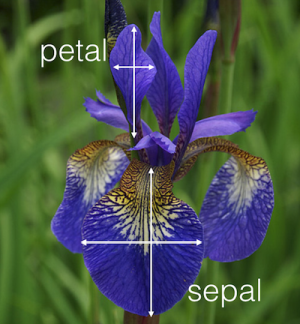
\includegraphics{assets/daten.assets/image_messung-16426070933692.png}
\caption{image (190)}
\end{figure}

\hypertarget{datensatz}{%
\subsection{Datensatz}\label{datensatz}}

Folgender - in der Community wohlbekannter - Datensatz liegt uns vor (Sie finden die Daten \href{https://syncandshare.lrz.de/getlink/fi89kxTJ5yLRaW5mnpyrofVK/Iris_p.xlsx}{hier}).

\begin{figure}
\centering
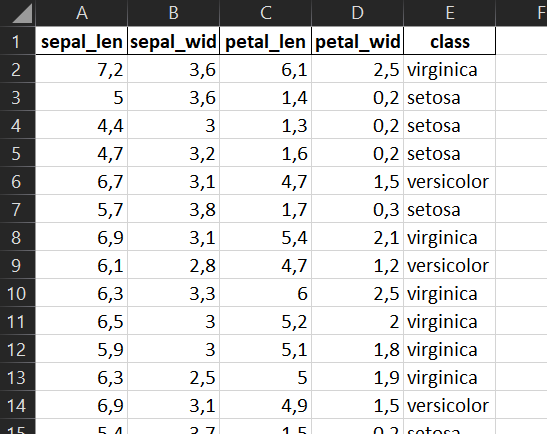
\includegraphics{assets/daten.assets/image-20211209101425856-16426070878651.png}
\caption{Iris-Datensatz}
\end{figure}

\hypertarget{datentypen}{%
\section{Datentypen}\label{datentypen}}

\hypertarget{elementare-datentypen}{%
\subsection{Elementare Datentypen}\label{elementare-datentypen}}

\hypertarget{zahlen}{%
\subsubsection{Zahlen}\label{zahlen}}

\hypertarget{strings}{%
\subsubsection{Strings}\label{strings}}

\hypertarget{logische-werte}{%
\subsubsection{Logische Werte}\label{logische-werte}}

\hypertarget{elementare-datentypen-in-python}{%
\subsubsection{Elementare Datentypen in Python}\label{elementare-datentypen-in-python}}

\hypertarget{komplexe-datentypen}{%
\subsection{Komplexe Datentypen}\label{komplexe-datentypen}}

\hypertarget{datum}{%
\subsubsection{Datum}\label{datum}}

\hypertarget{uhrzeit}{%
\subsubsection{Uhrzeit}\label{uhrzeit}}

\hypertarget{bilder}{%
\subsubsection{Bilder}\label{bilder}}

\hypertarget{komplexe-datentypen-in-python}{%
\subsubsection{Komplexe Datentypen in Python}\label{komplexe-datentypen-in-python}}

\hypertarget{skalenniveaus}{%
\section{Skalenniveaus}\label{skalenniveaus}}

\hypertarget{uxfcberblick}{%
\subsection{Überblick}\label{uxfcberblick}}

\begin{longtable}[]{@{}
  >{\raggedright\arraybackslash}p{(\columnwidth - 8\tabcolsep) * \real{0.0563}}
  >{\raggedright\arraybackslash}p{(\columnwidth - 8\tabcolsep) * \real{0.0915}}
  >{\raggedright\arraybackslash}p{(\columnwidth - 8\tabcolsep) * \real{0.4225}}
  >{\raggedright\arraybackslash}p{(\columnwidth - 8\tabcolsep) * \real{0.1268}}
  >{\raggedright\arraybackslash}p{(\columnwidth - 8\tabcolsep) * \real{0.3028}}@{}}
\toprule
\begin{minipage}[b]{\linewidth}\raggedright
Scale
\end{minipage} & \begin{minipage}[b]{\linewidth}\raggedright
Operations
\end{minipage} & \begin{minipage}[b]{\linewidth}\raggedright
Description
\end{minipage} & \begin{minipage}[b]{\linewidth}\raggedright
Statistics
\end{minipage} & \begin{minipage}[b]{\linewidth}\raggedright
Example
\end{minipage} \\
\midrule
\endhead
Nominal & \(=, \neq\) & values have no natural order; they describe unordered categories & Mode (Modus) & München, Hamburg, Essen \\
Ordinal & \(<, >\) & values have a defined order; difference of values is undefined or has no clear or meaningful definition & Median & Schulnoten, Tabellenplatz in der Bundesliga \\
Interval & \(+,-\) & differences of values have the same meaning; adding provides useful results; zero point is not naturally/globally defined & Mean & Temperatur \\
Ratio & \(\cdot , /\) & zero point is naturally defined & (Generalized) Mean & Alter \\
\bottomrule
\end{longtable}

Bemerkungen:

\begin{enumerate}
\def\labelenumi{\arabic{enumi}.}
\item
  Skalenniveaus sind nicht immer klar zuzuordnen.
\item
  Aus nominalen Datenskalen lassen sich stets \emph{künstliche Ordnungen} (und damit ordinale Datenskalen) definieren.
\item
  Bilden sie keine Mittelwerte auf Daten mit ordinalen Datenskalen!
\item
  Nominale und ordinale Datenskalen heißen auch \emph{kategorisch} oder \emph{qualitativ}.
\item
  Intervall und Ratio-Datenskalen heißen auch \emph{metrisch}.
\end{enumerate}

Ergänzend: \href{https://www.statistikpsychologie.de/skalenniveaus/}{Die fünf Skalenniveaus: Einfach und verständlich erklärt (statistikpsychologie.de)}

\hypertarget{skalenniveaus-im-iris-datensatz}{%
\subsection{Skalenniveaus im Iris-Datensatz}\label{skalenniveaus-im-iris-datensatz}}

\begin{figure}
\centering
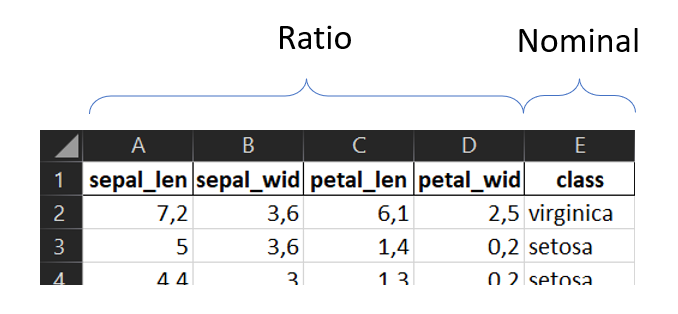
\includegraphics{assets/daten.assets/image-20211209145313372.png}
\caption{Skalenniveaus bei Iris}
\end{figure}

\hypertarget{von-nominal-zu-ordinal}{%
\paragraph{Von Nominal zu Ordinal}\label{von-nominal-zu-ordinal}}

Wir werden später folgende eindeutige Zuordnung treffen:

\begin{longtable}[]{@{}cc@{}}
\toprule
Nominaler Wert & Ordinaler Wert \\
\midrule
\endhead
setosa & 0 \\
versicolor & 1 \\
virginica & 2 \\
\bottomrule
\end{longtable}

\hypertarget{daten-1}{%
\chapter{Daten}\label{daten-1}}

\hypertarget{der-iris-datensatz-1}{%
\section{Der Iris-Datensatz}\label{der-iris-datensatz-1}}

Der Iris-Datensatz enthält Messungen von jeweils 50 Blüten zu drei verschiedenen Lilien-Arten (setosa, versicolor, virginica)

\begin{figure}
\centering
\includegraphics{assets/daten.assets/Download.png}
\caption{Download}
\end{figure}

Gemessen werden pro \href{https://de.wikipedia.org/wiki/Bl\%C3\%BCte}{Blüte}in cm 

\begin{itemize}
\tightlist
\item
  die Länge und Breite des Kronblattes (Petalum, petal) sowie 
\item
  die Länge und Breite des Kelchblattes (Sepalum, sepal)
\end{itemize}

\begin{figure}
\centering
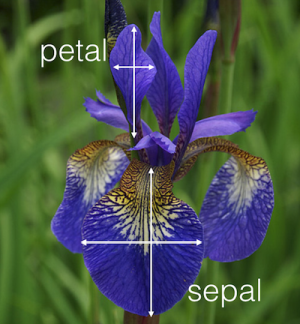
\includegraphics{assets/daten.assets/image_messung-16426070933692.png}
\caption{image (190)}
\end{figure}

\hypertarget{datensatz-1}{%
\subsection{Datensatz}\label{datensatz-1}}

Folgender - in der Community wohlbekannter - Datensatz liegt uns vor (Sie finden die Daten \href{https://syncandshare.lrz.de/getlink/fi89kxTJ5yLRaW5mnpyrofVK/Iris_p.xlsx}{hier}).

\begin{figure}
\centering
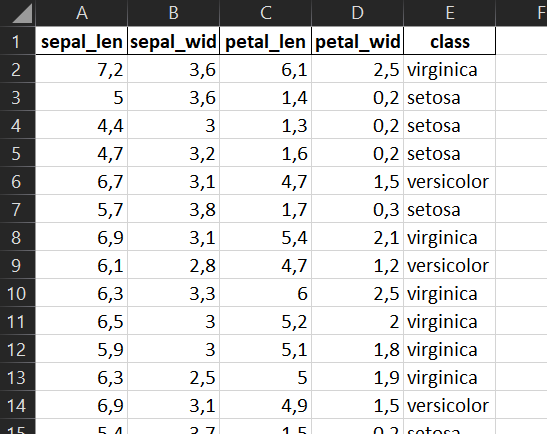
\includegraphics{assets/daten.assets/image-20211209101425856-16426070878651.png}
\caption{Iris-Datensatz}
\end{figure}

\hypertarget{datentypen-1}{%
\section{Datentypen}\label{datentypen-1}}

\hypertarget{elementare-datentypen-1}{%
\subsection{Elementare Datentypen}\label{elementare-datentypen-1}}

\hypertarget{zahlen-1}{%
\subsubsection{Zahlen}\label{zahlen-1}}

\hypertarget{strings-1}{%
\subsubsection{Strings}\label{strings-1}}

\hypertarget{logische-werte-1}{%
\subsubsection{Logische Werte}\label{logische-werte-1}}

\hypertarget{elementare-datentypen-in-python-1}{%
\subsubsection{Elementare Datentypen in Python}\label{elementare-datentypen-in-python-1}}

\hypertarget{komplexe-datentypen-1}{%
\subsection{Komplexe Datentypen}\label{komplexe-datentypen-1}}

\hypertarget{datum-1}{%
\subsubsection{Datum}\label{datum-1}}

\hypertarget{uhrzeit-1}{%
\subsubsection{Uhrzeit}\label{uhrzeit-1}}

\hypertarget{bilder-1}{%
\subsubsection{Bilder}\label{bilder-1}}

\hypertarget{komplexe-datentypen-in-python-1}{%
\subsubsection{Komplexe Datentypen in Python}\label{komplexe-datentypen-in-python-1}}

\hypertarget{skalenniveaus-1}{%
\section{Skalenniveaus}\label{skalenniveaus-1}}

\hypertarget{uxfcberblick-1}{%
\subsection{Überblick}\label{uxfcberblick-1}}

\begin{longtable}[]{@{}
  >{\raggedright\arraybackslash}p{(\columnwidth - 8\tabcolsep) * \real{0.0563}}
  >{\raggedright\arraybackslash}p{(\columnwidth - 8\tabcolsep) * \real{0.0915}}
  >{\raggedright\arraybackslash}p{(\columnwidth - 8\tabcolsep) * \real{0.4225}}
  >{\raggedright\arraybackslash}p{(\columnwidth - 8\tabcolsep) * \real{0.1268}}
  >{\raggedright\arraybackslash}p{(\columnwidth - 8\tabcolsep) * \real{0.3028}}@{}}
\toprule
\begin{minipage}[b]{\linewidth}\raggedright
Scale
\end{minipage} & \begin{minipage}[b]{\linewidth}\raggedright
Operations
\end{minipage} & \begin{minipage}[b]{\linewidth}\raggedright
Description
\end{minipage} & \begin{minipage}[b]{\linewidth}\raggedright
Statistics
\end{minipage} & \begin{minipage}[b]{\linewidth}\raggedright
Example
\end{minipage} \\
\midrule
\endhead
Nominal & \(=, \neq\) & values have no natural order; they describe unordered categories & Mode (Modus) & München, Hamburg, Essen \\
Ordinal & \(<, >\) & values have a defined order; difference of values is undefined or has no clear or meaningful definition & Median & Schulnoten, Tabellenplatz in der Bundesliga \\
Interval & \(+,-\) & differences of values have the same meaning; adding provides useful results; zero point is not naturally/globally defined & Mean & Temperatur \\
Ratio & \(\cdot , /\) & zero point is naturally defined & (Generalized) Mean & Alter \\
\bottomrule
\end{longtable}

Bemerkungen:

\begin{enumerate}
\def\labelenumi{\arabic{enumi}.}
\item
  Skalenniveaus sind nicht immer klar zuzuordnen.
\item
  Aus nominalen Datenskalen lassen sich stets \emph{künstliche Ordnungen} (und damit ordinale Datenskalen) definieren.
\item
  Bilden sie keine Mittelwerte auf Daten mit ordinalen Datenskalen!
\item
  Nominale und ordinale Datenskalen heißen auch \emph{kategorisch} oder \emph{qualitativ}.
\item
  Intervall und Ratio-Datenskalen heißen auch \emph{metrisch}.
\end{enumerate}

Ergänzend: \href{https://www.statistikpsychologie.de/skalenniveaus/}{Die fünf Skalenniveaus: Einfach und verständlich erklärt (statistikpsychologie.de)}

\hypertarget{skalenniveaus-im-iris-datensatz-1}{%
\subsection{Skalenniveaus im Iris-Datensatz}\label{skalenniveaus-im-iris-datensatz-1}}

\begin{figure}
\centering
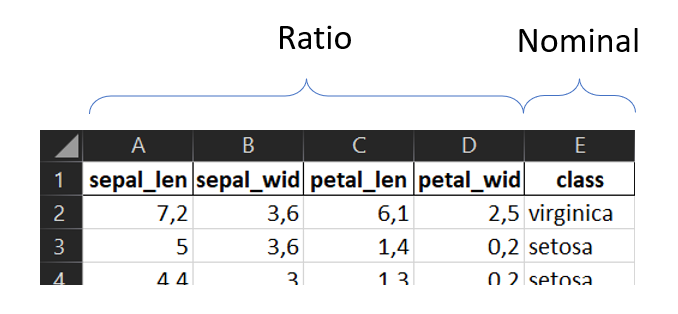
\includegraphics{assets/daten.assets/image-20211209145313372.png}
\caption{Skalenniveaus bei Iris}
\end{figure}

\hypertarget{von-nominal-zu-ordinal-1}{%
\paragraph{Von Nominal zu Ordinal}\label{von-nominal-zu-ordinal-1}}

Wir werden später folgende eindeutige Zuordnung treffen:

\begin{longtable}[]{@{}cc@{}}
\toprule
Nominaler Wert & Ordinaler Wert \\
\midrule
\endhead
setosa & 0 \\
versicolor & 1 \\
virginica & 2 \\
\bottomrule
\end{longtable}

\hypertarget{iris-datensatz}{%
\chapter{Iris-Datensatz}\label{iris-datensatz}}

\hypertarget{einfuxfchrung}{%
\section{Einführung}\label{einfuxfchrung}}

Der Iris-Datensatz enthält Messungen von jeweils 50 Blüten zu drei verschiedenen Lilien-Arten (setosa, versicolor, virginica)

\begin{figure}
\centering
\includegraphics[width=1\textwidth,height=\textheight]{assets/Download.png}
\caption[Iris-Arten]{Iris-Arten\footnotemark{}}
\end{figure}
\footnotetext{Quelle: Wikipedia}

Gemessen werden pro \href{https://de.wikipedia.org/wiki/Bl\%C3\%BCte}{Blüte} in cm 

\begin{itemize}
\tightlist
\item
  die Länge und Breite des Kronblattes (Petalum, petal) sowie 
\item
  die Länge und Breite des Kelchblattes (Sepalum, sepal)
\end{itemize}

\begin{figure}
\centering
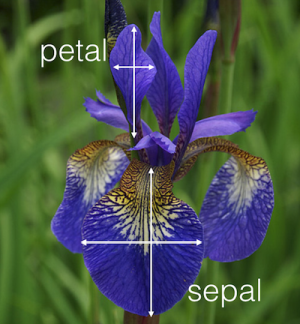
\includegraphics{assets/image_messung.png}
\caption[Petal und Sepal]{Petal und Sepal\footnotemark{}}
\end{figure}
\footnotetext{Quelle:xxx}

\hypertarget{datensatz-2}{%
\section{Datensatz}\label{datensatz-2}}

Folgender - in der Community wohlbekannter - Datensatz liegt uns vor (Sie finden die Daten \href{https://syncandshare.lrz.de/getlink/fi89kxTJ5yLRaW5mnpyrofVK/Iris_p.xlsx}{hier}).

\begin{figure}
\centering
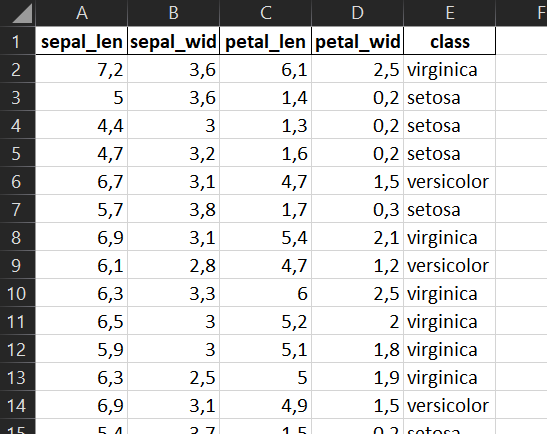
\includegraphics[width=0.6\textwidth,height=\textheight]{assets/image-20211209101425856.png}
\caption[Iris-Datensatz ]{Iris-Datensatz \footnotemark{}}
\end{figure}
\footnotetext{Fussnote}

Lorem ipsum dolor sit amet consectetur adipiscing elit sollicitudin lacus, dictumst fames condimentum mus penatibus aliquet phasellus lobortis, eleifend quam ligula eros tempus turpis proin dui. Convallis ridiculus vehicula vivamus facilisis nec proin et nostra sociis, nascetur in mollis felis accumsan nibh posuere dictum ad, lacinia placerat amet sed elementum magnis aptent vel. Sit posuere vivamus ultricies rutrum proin magnis inceptos ante mollis justo gravida, taciti condimentum adipiscing turpis habitasse facilisi fermentum cras maecenas vitae, libero lectus faucibus aptent urna etiam eget enim duis parturient. Ridiculus nisl class pellentesque magna orci sapien libero, potenti condimentum fames ipsum etiam semper, habitant vehicula amet lacinia praesent consequat. Conubia vestibulum nascetur potenti pretium massa magna feugiat hac, mattis commodo justo interdum libero donec egestas sed netus, lacus ac at dignissim sit amet platea. In posuere risus ipsum rutrum porta diam, sollicitudin congue eleifend interdum convallis penatibus est, pretium aliquam donec magna dictumst. Ac neque iaculis scelerisque euismod nec augue, enim ultricies fames vitae diam tristique, accumsan dictum ultrices quis ipsum. Potenti curabitur aliquet orci facilisi mi nam primis, diam massa augue et sem viverra laoreet, lacinia rhoncus magnis praesent leo vulputate.

Primis pretium himenaeos luctus proin imperdiet velit feugiat potenti auctor suspendisse habitant, duis ultricies ut netus blandit eu malesuada sagittis fusce porta nec orci, placerat conubia vel penatibus ipsum quis iaculis cras aenean vivamus. Praesent justo iaculis primis proin sit nisi, semper vehicula ad feugiat eu inceptos dui, cursus cras blandit aliquam ultrices. Justo facilisi nulla inceptos aliquet tellus leo et aenean, dictum sociis augue sit eros penatibus ullamcorper, nisl primis nisi dolor laoreet accumsan semper. Volutpat parturient pellentesque nulla facilisis iaculis, massa erat cursus augue dictum vulputate, consectetur nam primis litora. Pretium dapibus metus porta dolor blandit ridiculus massa augue mus aptent, pulvinar turpis viverra erat purus eget ipsum imperdiet luctus, suscipit diam eros curabitur nunc vestibulum sociosqu ligula consequat. Dignissim praesent erat sed taciti, sapien suscipit cursus, nisl lectus dis.

Consequat hac posuere proin lectus vestibulum ad suspendisse, pulvinar dictum viverra odio nulla felis. Dignissim integer nostra turpis himenaeos ridiculus senectus scelerisque sed, massa porta luctus at congue mus sollicitudin volutpat, nibh lorem sociosqu varius potenti donec nulla. Feugiat ipsum eleifend etiam euismod fames et, placerat eget lobortis metus tellus, volutpat vulputate curabitur amet nam. Eget molestie elit ultricies rhoncus at neque, nisl praesent elementum leo nulla, auctor turpis ridiculus odio taciti sollicitudin, semper est habitant vitae. Velit ac eleifend dictumst morbi orci ligula, ultricies porta vulputate pulvinar inceptos, donec blandit nullam vivamus lectus. Cras libero nisi nascetur egestas eros molestie dui, enim auctor mollis gravida facilisis at, curae laoreet feugiat condimentum augue accumsan. Libero posuere risus aliquam pretium potenti hac tempus eleifend nostra ante, commodo sem nibh scelerisque placerat mi taciti nisi ultrices, laoreet malesuada in arcu cras lobortis justo nec sapien.

Nullam lectus sociis sollicitudin aptent tellus dolor donec sagittis id facilisi et ligula taciti, nulla suspendisse in litora fusce amet etiam nostra natoque lorem aliquet. Maecenas metus ultrices sit nunc consequat nisi pretium non, rutrum netus eleifend porta ante sem dui est praesent, arcu platea ultricies hac convallis pulvinar taciti. Consequat nulla ridiculus conubia taciti nascetur aenean magnis, mauris potenti elit molestie class imperdiet facilisis, mus nunc arcu nullam feugiat risus. Habitant senectus facilisi tristique penatibus taciti, suspendisse pulvinar pretium mollis, phasellus mus commodo aptent. Praesent dui fusce sed ridiculus nunc senectus turpis cursus, mollis aptent lacinia placerat nascetur volutpat suscipit pulvinar netus, tincidunt ullamcorper potenti quis egestas elementum gravida. Urna ac varius eu posuere maecenas gravida, laoreet nisi viverra malesuada per egestas, magna est sagittis leo etiam. Ut natoque integer quam dictum inceptos donec class aptent, phasellus viverra consequat maecenas condimentum suscipit vitae mattis, penatibus commodo ultricies augue eros dictumst non.

\hypertarget{skalenniveaus-2}{%
\chapter{Skalenniveaus}\label{skalenniveaus-2}}

You can add parts to organize one or more book chapters together. Parts can be inserted at the top of an .Rmd file, before the first-level chapter heading in that same file.

Add a numbered part: \texttt{\#\ (PART)\ Act\ one\ \{-\}} (followed by \texttt{\#\ A\ chapter})

Add an unnumbered part: \texttt{\#\ (PART\textbackslash{}*)\ Act\ one\ \{-\}} (followed by \texttt{\#\ A\ chapter})

Add an appendix as a special kind of un-numbered part: \texttt{\#\ (APPENDIX)\ Other\ stuff\ \{-\}} (followed by \texttt{\#\ A\ chapter}). Chapters in an appendix are prepended with letters instead of numbers.

Lorem ipsum dolor sit amet consectetur adipiscing elit sollicitudin lacus, dictumst fames condimentum mus penatibus aliquet phasellus lobortis, eleifend quam ligula eros tempus turpis proin dui. Convallis ridiculus vehicula vivamus facilisis nec proin et nostra sociis, nascetur in mollis felis accumsan nibh posuere dictum ad, lacinia placerat amet sed elementum magnis aptent vel. Sit posuere vivamus ultricies rutrum proin magnis inceptos ante mollis justo gravida, taciti condimentum adipiscing turpis habitasse facilisi fermentum cras maecenas vitae, libero lectus faucibus aptent urna etiam eget enim duis parturient. Ridiculus nisl class pellentesque magna orci sapien libero, potenti condimentum fames ipsum etiam semper, habitant vehicula amet lacinia praesent consequat. Conubia vestibulum nascetur potenti pretium massa magna feugiat hac, mattis commodo justo interdum libero donec egestas sed netus, lacus ac at dignissim sit amet platea. In posuere risus ipsum rutrum porta diam, sollicitudin congue eleifend interdum convallis penatibus est, pretium aliquam donec magna dictumst. Ac neque iaculis scelerisque euismod nec augue, enim ultricies fames vitae diam tristique, accumsan dictum ultrices quis ipsum. Potenti curabitur aliquet orci facilisi mi nam primis, diam massa augue et sem viverra laoreet, lacinia rhoncus magnis praesent leo vulputate.

Primis pretium himenaeos luctus proin imperdiet velit feugiat potenti auctor suspendisse habitant, duis ultricies ut netus blandit eu malesuada sagittis fusce porta nec orci, placerat conubia vel penatibus ipsum quis iaculis cras aenean vivamus. Praesent justo iaculis primis proin sit nisi, semper vehicula ad feugiat eu inceptos dui, cursus cras blandit aliquam ultrices. Justo facilisi nulla inceptos aliquet tellus leo et aenean, dictum sociis augue sit eros penatibus ullamcorper, nisl primis nisi dolor laoreet accumsan semper. Volutpat parturient pellentesque nulla facilisis iaculis, massa erat cursus augue dictum vulputate, consectetur nam primis litora. Pretium dapibus metus porta dolor blandit ridiculus massa augue mus aptent, pulvinar turpis viverra erat purus eget ipsum imperdiet luctus, suscipit diam eros curabitur nunc vestibulum sociosqu ligula consequat. Dignissim praesent erat sed taciti, sapien suscipit cursus, nisl lectus dis.

Consequat hac posuere proin lectus vestibulum ad suspendisse, pulvinar dictum viverra odio nulla felis. Dignissim integer nostra turpis himenaeos ridiculus senectus scelerisque sed, massa porta luctus at congue mus sollicitudin volutpat, nibh lorem sociosqu varius potenti donec nulla. Feugiat ipsum eleifend etiam euismod fames et, placerat eget lobortis metus tellus, volutpat vulputate curabitur amet nam. Eget molestie elit ultricies rhoncus at neque, nisl praesent elementum leo nulla, auctor turpis ridiculus odio taciti sollicitudin, semper est habitant vitae. Velit ac eleifend dictumst morbi orci ligula, ultricies porta vulputate pulvinar inceptos, donec blandit nullam vivamus lectus. Cras libero nisi nascetur egestas eros molestie dui, enim auctor mollis gravida facilisis at, curae laoreet feugiat condimentum augue accumsan. Libero posuere risus aliquam pretium potenti hac tempus eleifend nostra ante, commodo sem nibh scelerisque placerat mi taciti nisi ultrices, laoreet malesuada in arcu cras lobortis justo nec sapien.

Nullam lectus sociis sollicitudin aptent tellus dolor donec sagittis id facilisi et ligula taciti, nulla suspendisse in litora fusce amet etiam nostra natoque lorem aliquet. Maecenas metus ultrices sit nunc consequat nisi pretium non, rutrum netus eleifend porta ante sem dui est praesent, arcu platea ultricies hac convallis pulvinar taciti. Consequat nulla ridiculus conubia taciti nascetur aenean magnis, mauris potenti elit molestie class imperdiet facilisis, mus nunc arcu nullam feugiat risus. Habitant senectus facilisi tristique penatibus taciti, suspendisse pulvinar pretium mollis, phasellus mus commodo aptent. Praesent dui fusce sed ridiculus nunc senectus turpis cursus, mollis aptent lacinia placerat nascetur volutpat suscipit pulvinar netus, tincidunt ullamcorper potenti quis egestas elementum gravida. Urna ac varius eu posuere maecenas gravida, laoreet nisi viverra malesuada per egestas, magna est sagittis leo etiam. Ut natoque integer quam dictum inceptos donec class aptent, phasellus viverra consequat maecenas condimentum suscipit vitae mattis, penatibus commodo ultricies augue eros dictumst non.

\hypertarget{blocks}{%
\chapter{Blocks}\label{blocks}}

\hypertarget{equations}{%
\section{Equations}\label{equations}}

Here is an equation.

\begin{equation} 
  f\left(k\right) = \binom{n}{k} p^k\left(1-p\right)^{n-k}
  \label{eq:binom}
\end{equation}

You may refer to using \texttt{\textbackslash{}@ref(eq:binom)}, like see Equation \eqref{eq:binom}.

\hypertarget{theorems-and-proofs}{%
\section{Theorems and proofs}\label{theorems-and-proofs}}

Labeled theorems can be referenced in text using \texttt{\textbackslash{}@ref(thm:tri)}, for example, check out this smart theorem \ref{thm:tri}.

\begin{theorem}
\protect\hypertarget{thm:tri}{}\label{thm:tri}For a right triangle, if \(c\) denotes the \emph{length} of the hypotenuse and \(a\) and \(b\) denote the lengths of the \textbf{other} two sides, we have \[a^2 + b^2 = c^2\]
\end{theorem}

Read more here \url{https://bookdown.org/yihui/bookdown/markdown-extensions-by-bookdown.html}.

\hypertarget{callout-blocks}{%
\section{Callout blocks}\label{callout-blocks}}

The \texttt{bs4\_book} theme also includes special callout blocks, like this \texttt{.rmdnote}.

You can use \textbf{markdown} inside a block.

\begin{Shaded}
\begin{Highlighting}[]
\FunctionTok{head}\NormalTok{(beaver1, }\AttributeTok{n =} \DecValTok{5}\NormalTok{)}
\CommentTok{\#\textgreater{}   day time  temp activ}
\CommentTok{\#\textgreater{} 1 346  840 36.33     0}
\CommentTok{\#\textgreater{} 2 346  850 36.34     0}
\CommentTok{\#\textgreater{} 3 346  900 36.35     0}
\CommentTok{\#\textgreater{} 4 346  910 36.42     0}
\CommentTok{\#\textgreater{} 5 346  920 36.55     0}
\end{Highlighting}
\end{Shaded}

It is up to the user to define the appearance of these blocks for LaTeX output.

You may also use: \texttt{.rmdcaution}, \texttt{.rmdimportant}, \texttt{.rmdtip}, or \texttt{.rmdwarning} as the block name.

The R Markdown Cookbook provides more help on how to use custom blocks to design your own callouts: \url{https://bookdown.org/yihui/rmarkdown-cookbook/custom-blocks.html}

\hypertarget{part-teil-b}{%
\part*{Teil B}\label{part-teil-b}}
\addcontentsline{toc}{part}{Teil B}

\hypertarget{sharing-your-book}{%
\chapter{Sharing your book}\label{sharing-your-book}}

\hypertarget{publishing}{%
\section{Publishing}\label{publishing}}

HTML books can be published online, see: \url{https://bookdown.org/yihui/bookdown/publishing.html}

\hypertarget{pages}{%
\section{404 pages}\label{pages}}

By default, users will be directed to a 404 page if they try to access a webpage that cannot be found. If you'd like to customize your 404 page instead of using the default, you may add either a \texttt{\_404.Rmd} or \texttt{\_404.md} file to your project root and use code and/or Markdown syntax.

\hypertarget{metadata-for-sharing}{%
\section{Metadata for sharing}\label{metadata-for-sharing}}

Bookdown HTML books will provide HTML metadata for social sharing on platforms like Twitter, Facebook, and LinkedIn, using information you provide in the \texttt{index.Rmd} YAML. To setup, set the \texttt{url} for your book and the path to your \texttt{cover-image} file. Your book's \texttt{title} and \texttt{description} are also used.

This \texttt{bs4\_book} provides enhanced metadata for social sharing, so that each chapter shared will have a unique description, auto-generated based on the content.

Specify your book's source repository on GitHub as the \texttt{repo} in the \texttt{\_output.yml} file, which allows users to view each chapter's source file or suggest an edit. Read more about the features of this output format here:

\url{https://pkgs.rstudio.com/bookdown/reference/bs4_book.html}

Or use:

\begin{Shaded}
\begin{Highlighting}[]
\NormalTok{?bookdown}\SpecialCharTok{::}\NormalTok{bs4\_book}
\end{Highlighting}
\end{Shaded}

\hypertarget{footnotes-and-citations}{%
\chapter{Footnotes and citations}\label{footnotes-and-citations}}

\hypertarget{footnotes}{%
\section{Footnotes}\label{footnotes}}

Footnotes are put inside the square brackets after a caret \texttt{\^{}{[}{]}}. Like this one \footnote{This is a footnote.}.

\hypertarget{citations}{%
\section{Citations}\label{citations}}

Reference items in your bibliography file(s) using \texttt{@key}.

For example, we are using the \textbf{bookdown} package \citep{R-bookdown} (check out the last code chunk in index.Rmd to see how this citation key was added) in this sample book, which was built on top of R Markdown and \textbf{knitr} \citep{xie2015} (this citation was added manually in an external file book.bib). Note that the \texttt{.bib} files need to be listed in the index.Rmd with the YAML \texttt{bibliography} key.

The \texttt{bs4\_book} theme makes footnotes appear inline when you click on them. In this example book, we added \texttt{csl:\ chicago-fullnote-bibliography.csl} to the \texttt{index.Rmd} YAML, and include the \texttt{.csl} file. To download a new style, we recommend: \url{https://www.zotero.org/styles/}

The RStudio Visual Markdown Editor can also make it easier to insert citations: \url{https://rstudio.github.io/visual-markdown-editing/\#/citations}

\hypertarget{template}{%
\chapter{Template}\label{template}}

You can add parts to organize one or more book chapters together. Parts can be inserted at the top of an .Rmd file, before the first-level chapter heading in that same file.

Add a numbered part: \texttt{\#\ (PART)\ Act\ one\ \{-\}} (followed by \texttt{\#\ A\ chapter})

Add an unnumbered part: \texttt{\#\ (PART\textbackslash{}*)\ Act\ one\ \{-\}} (followed by \texttt{\#\ A\ chapter})

Add an appendix as a special kind of un-numbered part: \texttt{\#\ (APPENDIX)\ Other\ stuff\ \{-\}} (followed by \texttt{\#\ A\ chapter}). Chapters in an appendix are prepended with letters instead of numbers.

\hypertarget{template-1}{%
\chapter{Template}\label{template-1}}

You can add parts to organize one or more book chapters together. Parts can be inserted at the top of an .Rmd file, before the first-level chapter heading in that same file.

Add a numbered part: \texttt{\#\ (PART)\ Act\ one\ \{-\}} (followed by \texttt{\#\ A\ chapter})

Add an unnumbered part: \texttt{\#\ (PART\textbackslash{}*)\ Act\ one\ \{-\}} (followed by \texttt{\#\ A\ chapter})

Add an appendix as a special kind of un-numbered part: \texttt{\#\ (APPENDIX)\ Other\ stuff\ \{-\}} (followed by \texttt{\#\ A\ chapter}). Chapters in an appendix are prepended with letters instead of numbers.

  \bibliography{book.bib,packages.bib}

\end{document}
